\documentclass[tikz,border=3pt]{standalone}
\usetikzlibrary{arrows.meta,decorations.markings}
\begin{document}
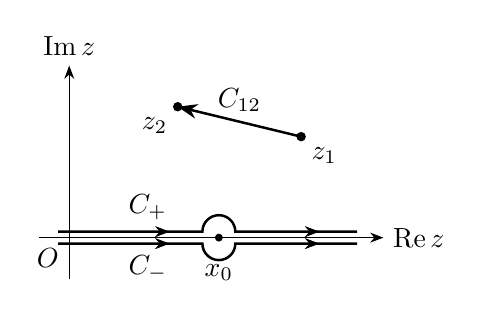
\begin{tikzpicture}[scale=0.95,>=Stealth,line width=0.9pt,
  mid/.style={postaction={decorate},decoration={markings,mark=at position #1 with {\arrow{Stealth[length=5pt]}}}}]
  % 座標軸
  \draw[line width=0.4pt,->] (-0.4,0) -- (4.2,0) node[right] {$\mathrm{Re}\,z$};
  \draw[line width=0.4pt,->] (0,-0.55) -- (0,2.3) node[above] {$\mathrm{Im}\,z$};
  \node[below left] at (0,0) {$O$};

  % x_0 の位置
  \def\xo{2.0}
  \fill (\xo,0) circle (1.5pt);
  \node[below,yshift=-6pt] at (\xo,0) {$x_0$};

  % 経路 C_+（わずかに上へずらし，x_0 を上半平面に迂回）
  \draw[mid=0.35,mid=0.88] (-0.15,0.08) -- (\xo-0.22,0.08)
    arc[start angle=180,end angle=0,radius=0.22] -- (3.85,0.08);
  \node[above] at (1.05,0.10) {$C_+$};

  % 経路 C_-（わずかに下へずらし，x_0 を下半平面に迂回）
  \draw[mid=0.35,mid=0.88] (-0.15,-0.08) -- (\xo-0.22,-0.08)
    arc[start angle=180,end angle=360,radius=0.22] -- (3.85,-0.08);
  \node[below] at (1.05,-0.10) {$C_-$};

  % 線分経路 C_{12}（z_1 から z_2 へ）
  \coordinate (z1) at (3.1,1.35);
  \coordinate (z2) at (1.45,1.75);
  \draw[->] (z1) -- (z2) node[midway,above] {$C_{12}$};
  \fill (z1) circle (1.8pt) node[below right] {$z_1$};
  \fill (z2) circle (1.8pt) node[below left] {$z_2$};
\end{tikzpicture}
\end{document}
